%-------------------------------------------------------------------------------------------------------------------
\section{SCM Workflow}
%-------------------------------------------------------------------------------------------------------------------

%-------------------------------------------------------------------------------------------------------------------
\begin{frame}

The SCM workflow describes the steps necessary to setup and run WRF-LIS (like the default workflow) using a single point domain.\\
\mbox{}\\
\emph{No chemistry is used}.
\mbox{}\\

\end{frame}

%-------------------------------------------------------------------------------------------------------------------
\begin{frame}

\centering
\textbf{NU-WRF Single Column Model (SCM) workflow.}
\begin{figure}[t]
\centering
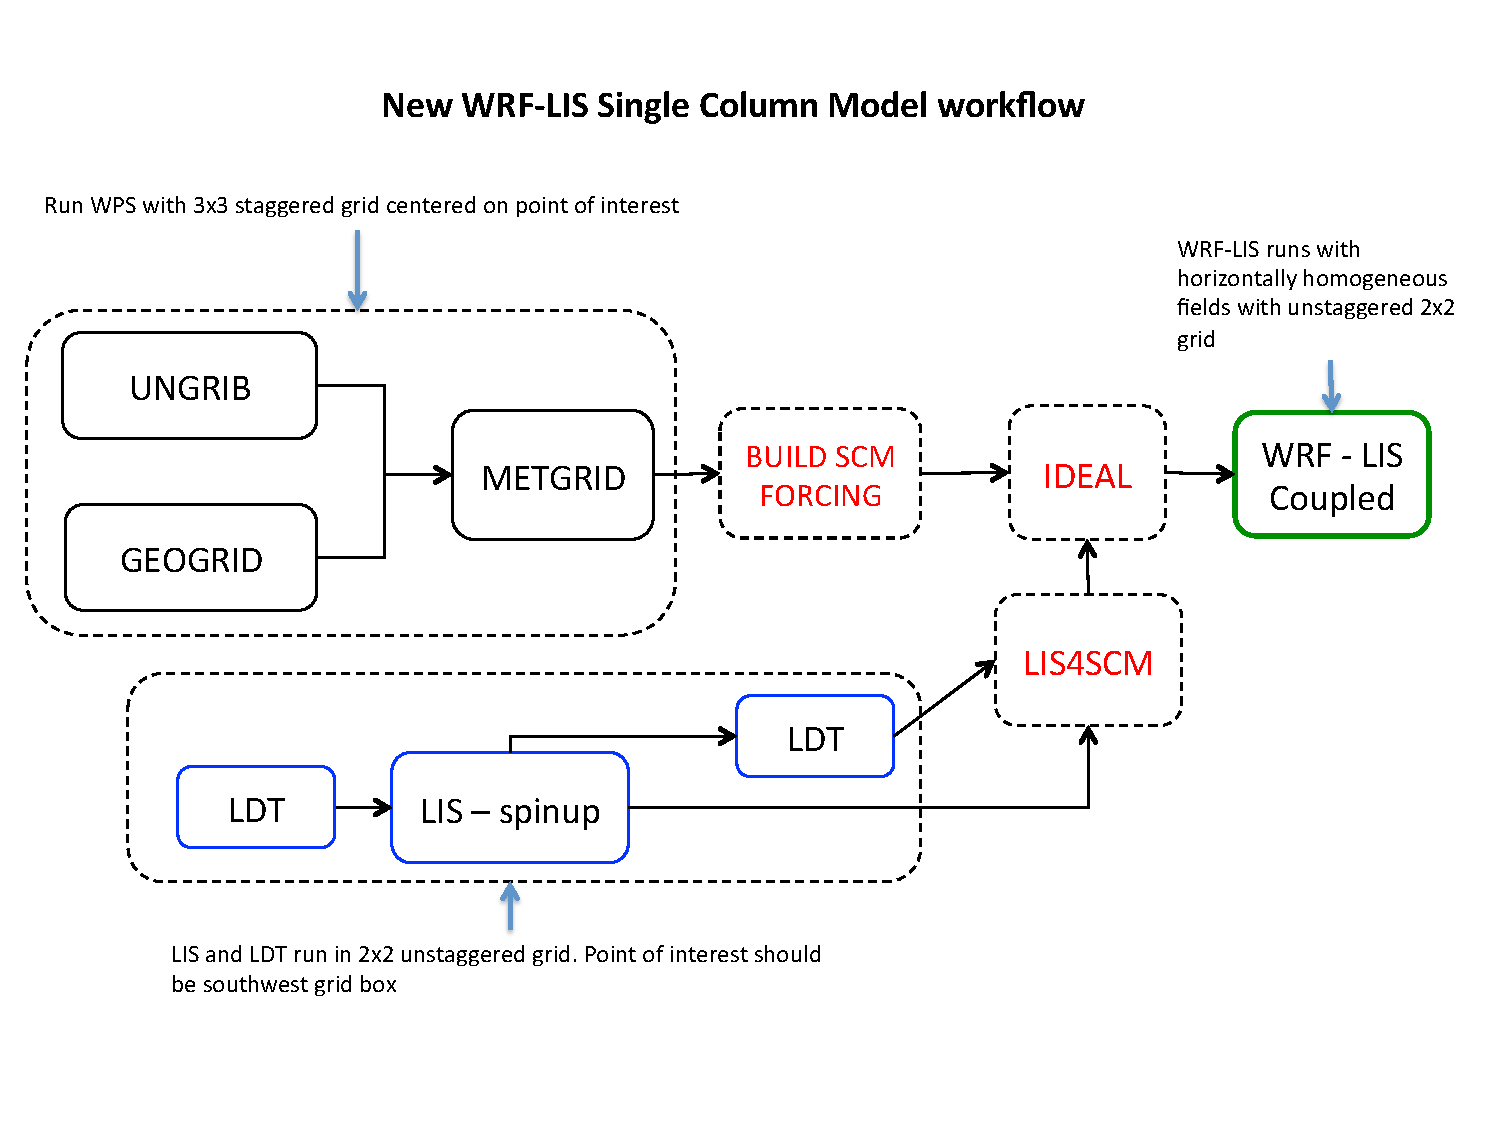
\includegraphics[scale=.4]{scm-workflow.pdf}
\end{figure}

\end{frame}

%-------------------------------------------------------------------------------------------------------------------
\begin{frame}[fragile]\frametitle{Required files for SCM workflow}

Copy the following files to \textbf{RUNDIR}:
\begin{lstlisting}
> export RUNDIR=/discover/nobackup/<my_user_id>/scratch/scm_workflow
> cp -r $PROJECTDIR/tutorial/scm_workflow $RUNDIR

Where:
common.reg : shared script with settings used by other scripts.
*.reg : scripts to run pre-processors and model.
namelist* : namelist files required by executables.
ungrib_input/* : GRIB atmospheric data for initial conditions used by UNGRIB component.
\end{lstlisting}

\end{frame}

%-------------------------------------------------------------------------------------------------------------------
\begin{frame}[fragile]
\frametitle{Required script changes}
\verbatimfont{\scriptsize}%
\begin{verbatim}
> cd $RUNDIR
\end{verbatim}
 Use your favorite editor to edit \textbf{common.reg} and change the values of NUWRFDIR and RUNDIR using the values set earlier.
\verbatimfont{\scriptsize}%
\begin{verbatim}
# *** Please make sure these settings are correct ***
# NUWRFDIR specifies the location of the NU-WRF source code
NUWRFDIR=<CHANGE THIS>
# RUNDIR specifies the location of the temporary run directory
RUNDIR=<CHANGE THIS>
\end{verbatim}
You may need to edit all the .reg files' account information and other settings. However, if you belong to group s0492 then the scripts should work without any modifications.
\verbatimfont{\scriptsize}%
\begin{verbatim}
Change account to appropriate SBU charge code:
#SBATCH --account s0942 
Change if you want to change number of nodes, hasw - to run on haswell nodes:
#SBATCH --ntasks=16 --constraint=hasw
Uncomment and set according to your needs and privileges:
##SBATCH --qos=high 
Uncomment (if desired) and substitute your e-mail here:
##SBATCH --mail-user=user@nasa.gov 
\end{verbatim}

\end{frame}

%-------------------------------------------------------------------------------------------------------------------
\begin{frame}[fragile]\frametitle{A note about namelists settings}

Things to keep in mind before we run NU-WRF components.
\mbox{}\\
\begin{itemize}
\item The length of the simulations is specified in the namelist files:
\begin{itemize}
\item In namelist.wps the length is determined by start\_date and end\_date
\item In namelist.input look for start\_ and end\_ fields. 
\item The dates in both namelists must be consistent.
\end{itemize}
\item The workflow is designed to work as-is. However, if you want to run for different dates:
\begin{itemize}
\item You must get the corresponding atmospheric data for initial conditions. 
\item Yo may need to modify the namelists. For example in namelist.input, make sure end\_day - start\_day = run\_days.
\end{itemize}
\item For \textbf{any} other changes please refer to the user's guide.
\end{itemize}
\end{frame}

%-------------------------------------------------------------------------------------------------------------------
\begin{frame}[fragile]\frametitle{GEOGRID}

\scriptsize{
GEOGRID interpolates static and climatological terrestrial data (land use, albedo, vegetation greenness, etc) to each WRF grid.
\begin{itemize}
\item Input: namelist.wps
\item Output: For \emph{N} domains (max\_dom in namelist.wps), \emph{N} geo\_em files will be created.
\end{itemize}\scriptsize}    
\hrulefill\par
To run GEOGRID:
\verbatimfont{\scriptsize}%
\begin{verbatim}
> cd $RUNDIR
> sbatch geogrid.reg
\end{verbatim}
When done, check for  "Successful completion"  string in the file geogrid.slurm.out.
geogrid.log file will also be created which can be used for tracking run failures or debugging.


\end{frame}

%-------------------------------------------------------------------------------------------------------------------
\begin{frame}[fragile]\frametitle{UNGRIB}

\footnotesize{
UNGRIB reads GRIB or GRIB2 files with dynamic meteorological and dynamic terrestrial data (soil moisture, soil temperature, sea surface temperature, sea ice, etc) and writes specific fields in a WPS intermediate format.
\begin{itemize}
\item Input: namelist.wps, ungrib\_input/* files.
\item Output: NARR* files.
\end{itemize}}
\scriptsize{\textbf{NOTE}: The GRIB input is referenced in the run script, run\_ungrib.bash:\\
      ./link\_grib.csh ungrib\_input/*\\
The UNGRIB output (NARR) is determined by the settings in the WPS namelist (namelist.wps). \\
}
\hrulefill\par
\footnotesize{To run:}
\begin{lstlisting}
> cd $RUNDIR
> ./ungrib.reg
\end{lstlisting}
When done, check for  "Successful completion"  string in the file ungrib.slurm.out. ungrib.log will also be created for tracking run failures or debugging.

\end{frame}

%-------------------------------------------------------------------------------------------------------------------
\begin{frame}[fragile]\frametitle{METGRID}

\footnotesize{
METGRID horizontally interpolates the output from UNGRIB to the WRF domains, and combines it with the
output from GEOGRID.
\begin{itemize}
\item Input: namelist.wps, NARR* files, geo\_em* files.
\item Output: Several met\_em* files corresponding to number of intervals (interval\_seconds) in simulation length (start/end dates).
\end{itemize}
}    
\hrulefill\par
\footnotesize{To run:}
\begin{lstlisting}
> cd $RUNDIR
> sbatch metgrid.reg
\end{lstlisting}
When done, check for  "Successful completion" string in the file metgrid.slurm.out. metgrid.log.nnnn (nnnn is the cpu number) files also be created for tracking run failures or debugging.


\end{frame}

%-------------------------------------------------------------------------------------------------------------------
\begin{frame}[fragile]\frametitle{BUILD\_SCM\_FORCING}

\footnotesize{
BUILD\_SCM\_FORCING scripts use WPS output and generate column initial conditions profile\_init.txt and surface\_init.txt. \\
Note that this script depends on NCL and on Discover one needs to load other/ncl-6.3.0-static.
\begin{itemize}
\item Input: WPS output, forcing\_file.cdl and several *.ncl files.
\item Output: profile\_init.txt, surface\_init.txt, and a directory, 2006-07-14\_00:00:00,  containing forcing\_file.nc and input\_sounding data.
\end{itemize}
}    
\hrulefill\par
\footnotesize{To run:}
\begin{lstlisting}
> cd $RUNDIR

Edit build_scm_forcing.bash: set metPath and forceArcRoot equal to RUNDIR value.

> ./build_scm_forcing.bash # runs in serial
\end{lstlisting}
After some other "messages" you should see "SUCCESS" printed on the terminal.
\end{frame}

%-------------------------------------------------------------------------------------------------------------------
\begin{frame}[fragile]\frametitle{LDT (pre-LIS)}

\footnotesize{
LDT processes data inputs for different surface models. In this use-case  we are using the Noah v3.6 land surface model.
\begin{itemize}
\item Input: ldt.config
\item Output: lis\_input* files for each NU-WRF domain.
\end{itemize}
}    
\hrulefill\par
\footnotesize{To run:}
\begin{lstlisting}
> cd $RUNDIR
> sbatch ldt_prelis.reg

When done, check for "Finished LDT run" string in the file ldt_log_prelis.0000
\end{lstlisting}

\end{frame}

%-------------------------------------------------------------------------------------------------------------------
\begin{frame}[fragile]\frametitle{LIS}

\footnotesize{
LIS  can be run from a cold start or from a restart. A cold start run is usually a multi-year simulation, not appropriate for a tutorial - though one can concoct a short spin up run for demo purposes. In the restart case we have to provide restart files as input (LIS\_RST* files) and the LIS run can be significantly shorter. Nevertheless,  the restart (and history) files have already been generated for this tutorial and the user can \textbf{skip} this step.
\mbox{}\\
If you want to run a LIS spin up for this case you may look at the default workflow and use those scripts and config files as a template.
}    

\end{frame}

%-------------------------------------------------------------------------------------------------------------------
\begin{frame}[fragile]\frametitle{LDT (post-LIS)}

\footnotesize{
After running LIS, it is necessary to rerun LDT in "NUWRF preprocessing for real" mode. This requires modifications to ldt.config to specify the static output file from LDT and the dynamic output file from LIS. Fields from both will be combined and written to a new netCDF output file for use by REAL
\begin{itemize}
\item Input: ldt.config
\item Output: lis4real\_input* files for each NU-WRF domain.
\end{itemize}
}    
\hrulefill\par
\footnotesize{To run:}
\begin{lstlisting}
> cd $RUNDIR
> sbatch ldt_postlis.reg

When done, check for "Finished LDT run" string in the file ldt_log_postlis.0000
\end{lstlisting}

\end{frame}


%-------------------------------------------------------------------------------------------------------------------
\begin{frame}[fragile]\frametitle{LIS4SCM}

\footnotesize{
LIS4SCM copies data from southwest grid point to remainder of LIS/LDT domain (becomes horizontally homogenous): LIS4SCM imposes identical lat/lon at each LIS point in the restart file.
\begin{itemize}
\item Input: namelist.lis4scm, LDT-LIS-LDT output
\item Output: Horizontally homogeneous lis\_input file (lis\_input.d01.nc)
\end{itemize}
}    
\hrulefill\par
\footnotesize{To run:}
\begin{lstlisting}
> cd $RUNDIR
> ./lis4scm.reg   # Note this runs in serial
\end{lstlisting}


\end{frame}

%-------------------------------------------------------------------------------------------------------------------
\begin{frame}[fragile]\frametitle{IDEAL}

\footnotesize{
IDEAL creates wrfinput file from text column data and homogeneous LIS/LDT file.
\begin{itemize}
\item Input: LIS4SCM output
\item Output: wrfinput file (wrfinput\_d01).
\end{itemize}
}    
\hrulefill\par
\footnotesize{To run:}
\begin{lstlisting}
> cd $RUNDIR
> sbatch ideal.reg
\end{lstlisting}

\end{frame}

%-------------------------------------------------------------------------------------------------------------------
\begin{frame}[fragile]\frametitle{WRF-LIS}

\footnotesize{
WRF-LIS reads wrfinput and the homogenous LIS restart file.
\begin{itemize}
\item Input: wrfinput file
\item Output: wrfoutput file.
\end{itemize}
}    
\hrulefill\par
\footnotesize{To run:}
\begin{lstlisting}
> cd $RUNDIR
> sbatch wrf.reg
\end{lstlisting}
\footnotesize{
\hrulefill\par       
Notes:
\begin{itemize}
\item Tested case uses periodic LBCs (thus, no wrfbdy file).
\item Tested case also used no forcing (no external advection, etc).
\item Tested case used dx = 1 km, dt = 6 sec (runs very fast!)
\end{itemize}
}    

\end{frame}

%-------------------------------------------------------------------------------------------------------------------
\begin{frame}[fragile]
\frametitle{Post-processing on Discover}

Using NCVIEW:

\begin{lstlisting}
WRF output files (NETCDF4) can be viewed using a special version of ncview installed on Discover:

/usr/local/other/SLES11.1/ncview/2.1.2/intel-12.1.0.233/bin/ncview <filename>
\end{lstlisting}

\end{frame}

%-------------------------------------------------------------------------------------------------------------------
\begin{frame}[fragile]
\frametitle{Post-processing on Discover}

Using RIP (NCAR graphics). Submit the \textbf{rip} job:
\begin{lstlisting}
> cd $RUNDIR
> ./rip.bash # (or use sbatch)
> idt filename.cgm # Substitute actual filename

rip.bash will run ripdp_wrfarw and rip to generate NCAR Graphics cgm files.
idt is a NCAR Graphics executable in $NCARG_ROOT/bin
Sample RIP plot specification tables are in $NUWRFDIR/scripts/rip and are looped through by rip.bash

See http://www2.mmm.ucar.edu/wrf/users/docs/ripug.htm for info on customizing plots with RIP. 
Minor changes to rip.bash may be necessary.
\end{lstlisting}

\end{frame}





